% Exact-run source: results/uniform_runs.csv (nine unique settings).
\begin{figure}[htbp]
\centering
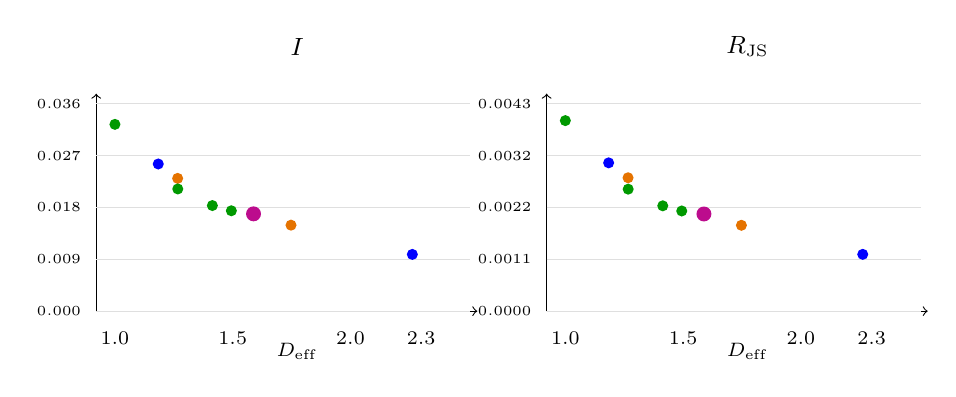
\begin{tikzpicture}[x=.88cm,y=.85cm]
\node[font=\small] at (3.60,4.85) {$I$};
\draw[->] (0.70,.9)--(6.20,.9);
\draw[->] (0.70,.9)--(0.70,4.15);
\draw[gray!25] (0.70,0.900)--(6.10,0.900);
\node[font=\tiny,anchor=east] at (0.62,0.900) {$0.000$};
\draw[gray!25] (0.70,1.675)--(6.10,1.675);
\node[font=\tiny,anchor=east] at (0.62,1.675) {$0.009$};
\draw[gray!25] (0.70,2.450)--(6.10,2.450);
\node[font=\tiny,anchor=east] at (0.62,2.450) {$0.018$};
\draw[gray!25] (0.70,3.225)--(6.10,3.225);
\node[font=\tiny,anchor=east] at (0.62,3.225) {$0.027$};
\draw[gray!25] (0.70,4.000)--(6.10,4.000);
\node[font=\tiny,anchor=east] at (0.62,4.000) {$0.036$};
\node[font=\scriptsize,anchor=north] at (0.970,.73) {$1.0$};
\node[font=\scriptsize,anchor=north] at (2.670,.73) {$1.5$};
\node[font=\scriptsize,anchor=north] at (4.370,.73) {$2.0$};
\node[font=\scriptsize,anchor=north] at (5.390,.73) {$2.3$};
\node[font=\scriptsize] at (3.60,.30) {$D_{\mathrm{eff}}$};
\fill[magenta!75!blue] (2.970,2.354) circle (2.7pt);
\fill[blue] (5.262,1.748) circle (2.0pt);
\fill[blue] (1.595,3.099) circle (2.0pt);
\fill[orange!90!black] (1.875,2.884) circle (2.0pt);
\fill[orange!90!black] (3.511,2.185) circle (2.0pt);
\fill[green!60!black] (0.970,3.691) circle (2.0pt);
\fill[green!60!black] (1.877,2.726) circle (2.0pt);
\fill[green!60!black] (2.376,2.478) circle (2.0pt);
\fill[green!60!black] (2.650,2.400) circle (2.0pt);
\node[font=\small] at (10.10,4.85) {$R_{\mathrm{JS}}$};
\draw[->] (7.20,.9)--(12.70,.9);
\draw[->] (7.20,.9)--(7.20,4.15);
\draw[gray!25] (7.20,0.900)--(12.60,0.900);
\node[font=\tiny,anchor=east] at (7.12,0.900) {$0.0000$};
\draw[gray!25] (7.20,1.675)--(12.60,1.675);
\node[font=\tiny,anchor=east] at (7.12,1.675) {$0.0011$};
\draw[gray!25] (7.20,2.450)--(12.60,2.450);
\node[font=\tiny,anchor=east] at (7.12,2.450) {$0.0022$};
\draw[gray!25] (7.20,3.225)--(12.60,3.225);
\node[font=\tiny,anchor=east] at (7.12,3.225) {$0.0032$};
\draw[gray!25] (7.20,4.000)--(12.60,4.000);
\node[font=\tiny,anchor=east] at (7.12,4.000) {$0.0043$};
\node[font=\scriptsize,anchor=north] at (7.470,.73) {$1.0$};
\node[font=\scriptsize,anchor=north] at (9.170,.73) {$1.5$};
\node[font=\scriptsize,anchor=north] at (10.870,.73) {$2.0$};
\node[font=\scriptsize,anchor=north] at (11.890,.73) {$2.3$};
\node[font=\scriptsize] at (10.10,.30) {$D_{\mathrm{eff}}$};
\fill[magenta!75!blue] (9.470,2.352) circle (2.7pt);
\fill[blue] (11.762,1.749) circle (2.0pt);
\fill[blue] (8.095,3.116) circle (2.0pt);
\fill[orange!90!black] (8.375,2.893) circle (2.0pt);
\fill[orange!90!black] (10.011,2.183) circle (2.0pt);
\fill[green!60!black] (7.470,3.747) circle (2.0pt);
\fill[green!60!black] (8.377,2.723) circle (2.0pt);
\fill[green!60!black] (8.876,2.474) circle (2.0pt);
\fill[green!60!black] (9.150,2.397) circle (2.0pt);
\end{tikzpicture}
\caption{رابطه مشاهده‌شده میان عمق مؤثر بازنمایی و هندسه کلاس‌ها در نه تنظیم سیاست یکنواخت. $I$ معیار جدایی مراکز و $R_{\mathrm{JS}}$ معیار پراکندگی درون‌کلاسی است. رنگ‌ها در نسخه برداری برای عوامل تغییر متفاوت‌اند؛ نقطه مبنا تنها یک اجرا محسوب می‌شود. این مقایسه مشاهده‌ای است و رابطه علّی یا بهینگی پارامترها را اثبات نمی‌کند.}
\label{fig:ch4-uniform-geometry-vs-depth}
\end{figure}
